\documentclass[12pt]{article}
\usepackage[utf8]{inputenc}
\usepackage[spanish]{babel}
\usepackage{ragged2e}

%Tabla
\usepackage{array}
\usepackage{booktabs}

%Fuente Personalizada
\usepackage{fontspec}
\setmainfont{Arial}

%Interlineado
\renewcommand{\baselinestretch}{1.5}

% Arquitectura de página:
\usepackage[left=2.54cm,right=2.54cm,top=2.54cm,bottom=2.54cm]{geometry}

% Paquete Imágenes
\usepackage{graphicx}
\graphicspath{ {images/} }
\usepackage{subfig}

%Pies de página y encabezado
\usepackage{fancyhdr}
\pagestyle{fancy}
\fancyhf{}
\lhead{\begin{picture}(0,0) \put(0,0){
\includegraphics[height=5mm]{Logo Simple.png}} \end{picture}}
\rhead{DevFest 2021}
\renewcommand{\headrulewidth}{0.5pt}
\cfoot{\thepage}
\lfoot{}

%Símbolos
\usepackage{eurosym}    %Euros \euros

\title{Dossier GDG}
\author{Google Developer Group, Jaén }
\date{Octubre 2021}


\begin{document}


\begin{titlepage}
\centering
\begin{figure}[h]
\vspace{3.5cm}
\centering

\includegraphics[scale=0.5]{LogoGDGJaenProvinciaFondoBlanco.png}
\end{figure}
\vspace{3cm}
{\scshape\Huge DEVFEST 2021\par}
\vspace{3cm}
{\itshape\Large \par}
\vfill
{\Large Google Developer Group of Jaén \par}
\vfill
{\Large Octubre 2021 \par}
\end{titlepage}


\newpage

\tableofcontents

\newpage
\section{¿Quiénes somos?}


GDG Jaén es una comunidad sin ánimo de lucro cuyo interés es fomentar las nuevas tecnologías en nuestra localidad y ayudar a los jienenses a encontrar personas con las que poder compartir sus intereses y proyectos.


Tenemos el honor de haber creado una comunidad con más de 900 desarrolladores posicionándonos como una de las comunidades más sólidas de la provincia y de toda Andalucía.


\begin{figure}[h]
    \centering
    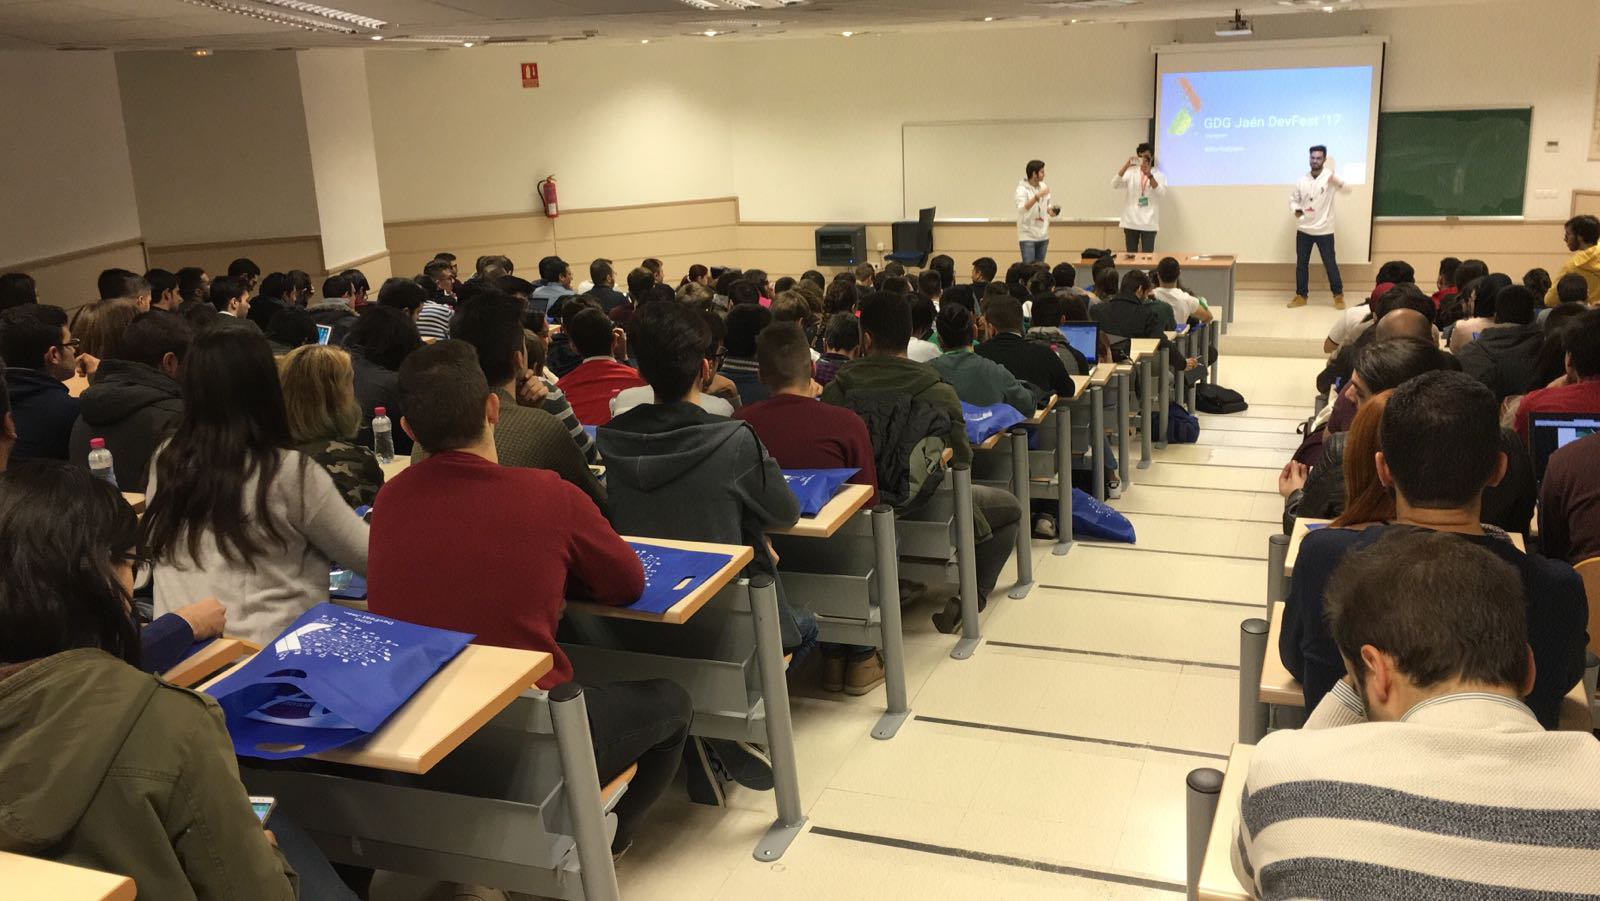
\includegraphics[width=0.7\textwidth]{people.jpeg}
    \caption{Inauguración DevFest 2018}
    \label{fig:my_label}
\end{figure}

Reunimos a programadores y entusiastas de la tecnología que deseen desarrollar soluciones de distinta índole, apoyándonos en buenas prácticas establecidas por Google, sin olvidar otras tecnologías innovadoras.


\section{Objetivos}
Nuestros objetivos como organización son:
\begin{enumerate}
    \item Promover el talento de nuestra ciudad.
    \item Dar a conocer la tecnología generada por la Universidad y las empresas de Jaén.
    \item Fomentar la creatividad, la actitud crítica y el desarrollo personal dentro de la provincia de Jaén.
    \item Conectar personas porque creemos que crecer con amigos es crecer dos veces.
    \item Acercar empresa y Universidad de modo que las empresas locales tengan acceso directo a estudiantes universitarios interesados en aprender.
    \item Fomentar la cooperación, el intercambio de ideas y la integración dentro de la comunidad.
\end{enumerate}

\section{¿Qué es el DevFest?}
DevFest es el evento anual más importante de la comunidad GDG llevado a cabo en todo el mundo por casi 900 grupos, el objetivo es acercar el conocimiento a nuestras comunidades locales uniendo, en una jornada, a los mejores ponentes técnicos.
\begin{figure}[h]
    \centering
    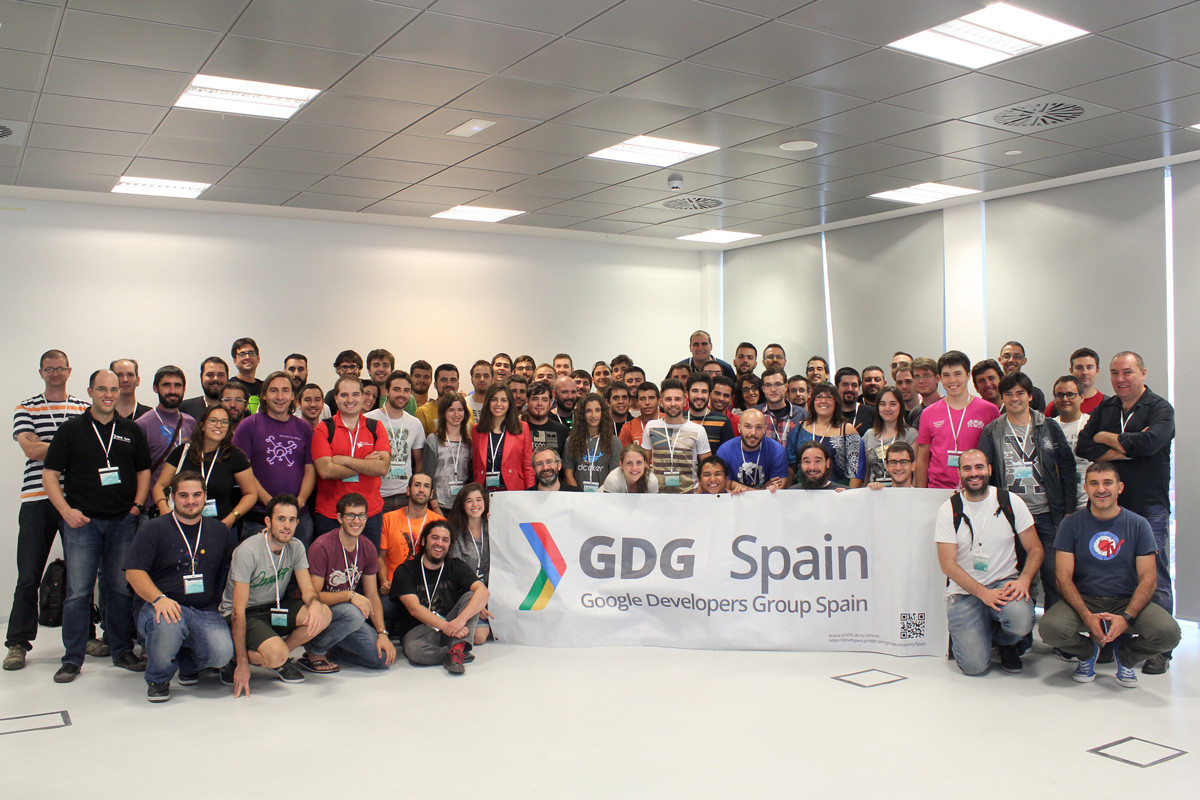
\includegraphics[width=0.75\textwidth]{GDG_Spain.jpg}
    \caption{GDG Spain}
    \label{fig:my_label}
\end{figure}
\subsection{Anteriores DevFest}
Nos encontramos este año ante el reto de nuestra $3^{a}$ edición del DevFest, tras el éxito cosechado en nuestras anteriores ediciones en las cuales tuvimos el placer de ser el GDG con el \textbf{DevFest más grande de España}, esperamos en esta edición seguir mejorando y creciendo.
\begin{figure}[h]
    \centering
    \includegraphics[width=0.7\textwidth]{Presentación.jpg}
    \caption{Inauguración DevFest 2018}
    \label{fig:my_label}
\end{figure}
Nuestra principal fuente de asistentes ha sido Twitter, otras redes sociales y el boca a boca de nuestros asistentes de ediciones anteriores. Gracias a esto en la pasada edición conseguimos atraer a 400 personas, lo que nos permitirá llegar a más gente en este año y mayor visibilidad para la organización y los patrocinadores.

Durante la anterior edición contamos con 20 ponentes que, durante todo un día, compartieron con todos sus conocimientos, repartidos en 5 tracks con distintas temáticas.

\begin{figure}
 \centering
  \subfloat[]{
   \label{f:gato}
    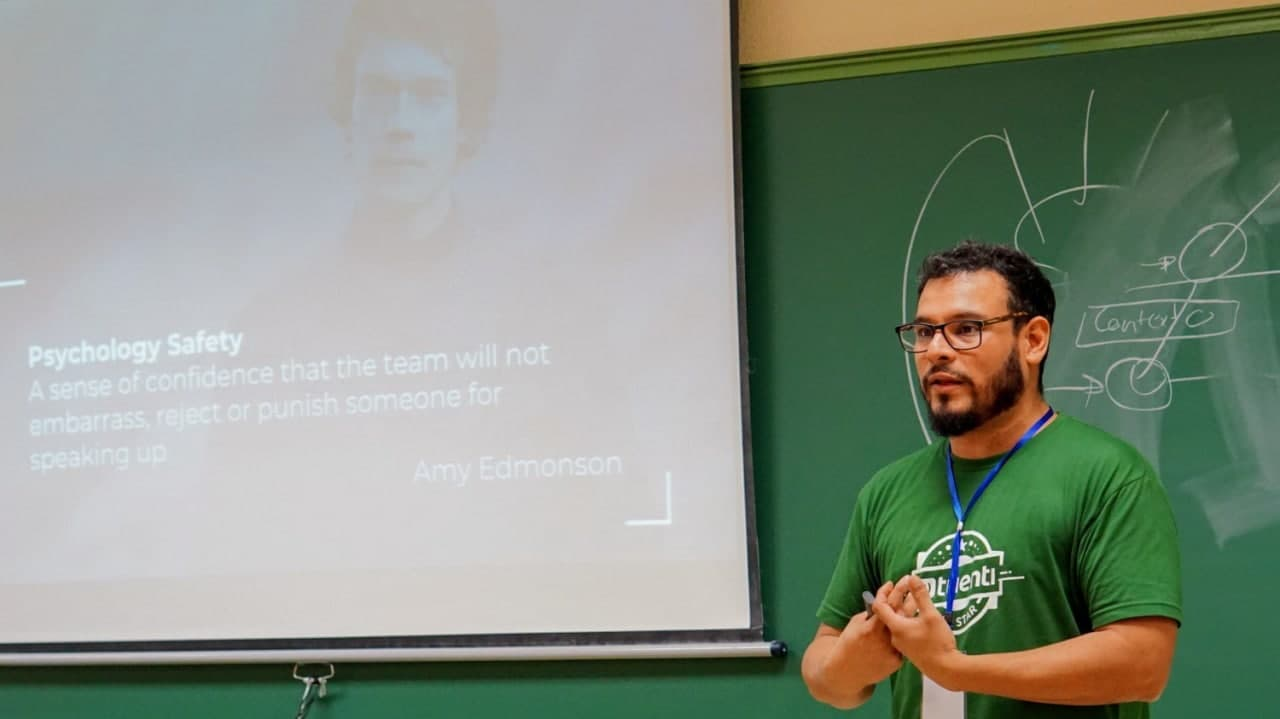
\includegraphics[width=0.45\textwidth]{Charla.jpg}}
  \subfloat[]{
   \label{f:tigre}
    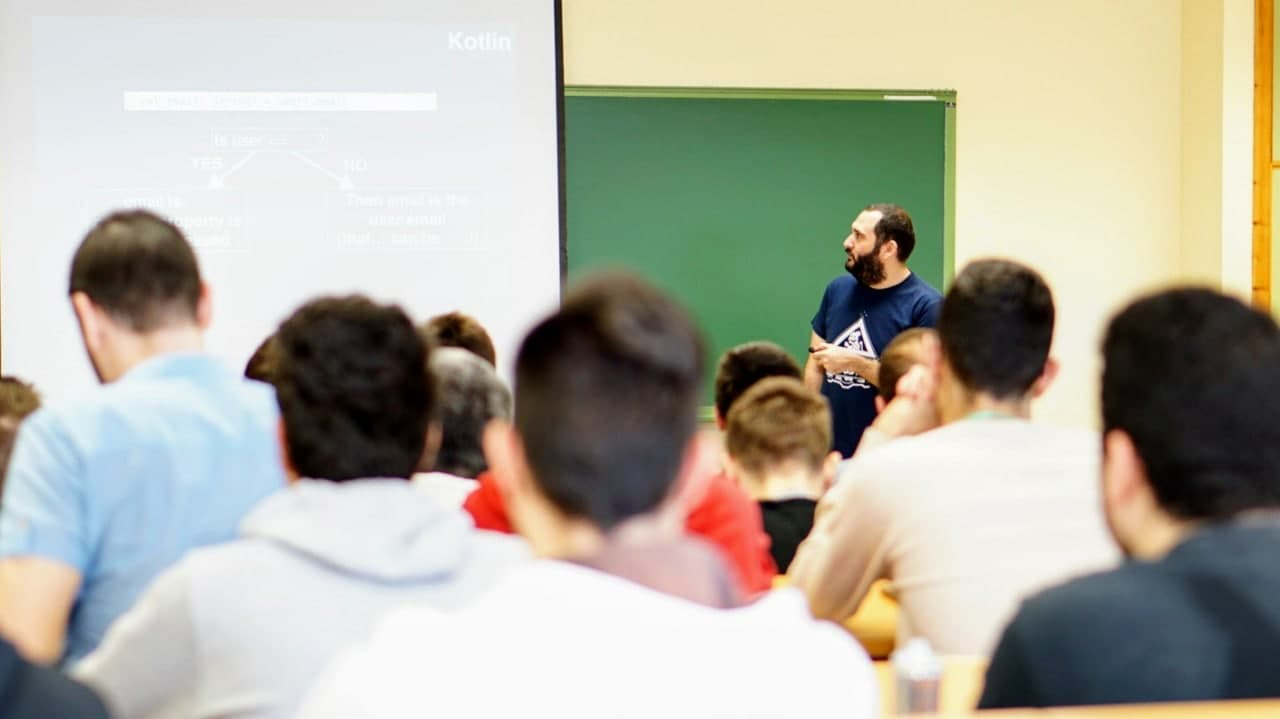
\includegraphics[width=0.45\textwidth]{Charla jorge.jpg}}
 \caption{Charlas DevFest}
 \label{f:animales}
\end{figure}
El hashtag usado durante el evento, \textbf{\#DevFestJaen}, cuenta con un impacto potencial de \textbf{73.071 veces visto} y un \textbf{alcance de 34.320 personas} y a nivel de prensa hemos sido cubiertos por la gran mayoría de medios locales online, como pueden ser: \textit{la contra de Jaén, hora Jaén, onda Jaén RTV, diario Jaén o campiña digital} y una parte importante de los medios de distribución física entre los que se incluyen algunos de los mencionados arriba, como diario Jaén.
\subsection{GDG}

La familia de GDG Jaén está formada por un equipo de 8 organizadores y organizadoras que trabajan durante el año para que DevFest salga adelante de la manera más exitosa posible. Para ello, también tenemos el apoyo de la Universidad de Jaén, más concretamente el vicerrectorado de Estudiantes y la Escuela Politécnica Superior, además del apoyo de Google. 
\begin{figure}[h]
    \centering
    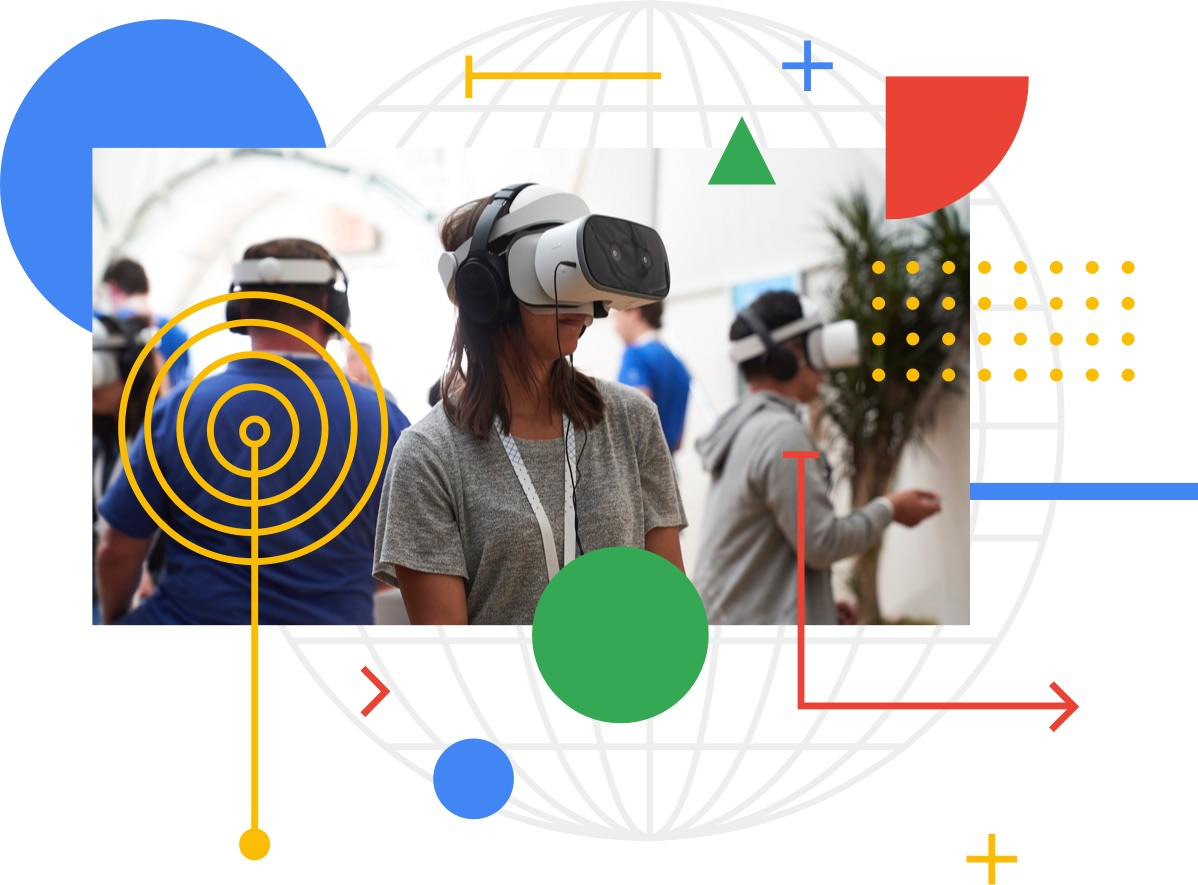
\includegraphics[width=0.7\textwidth]{assets.jpeg}
    \caption{Realidad Virtual}
    \label{fig:my_label}
\end{figure}
\subsection{Temática}
Nuestro evento suele estar estructurado en diferentes tracks que contienen actividades como charlas y talleres que se desarrollan de manera paralela durante la mañana y la tarde para que así nuestros asistentes tengan un abanico de posibilidades.
\begin{figure}[h]
    \centering
    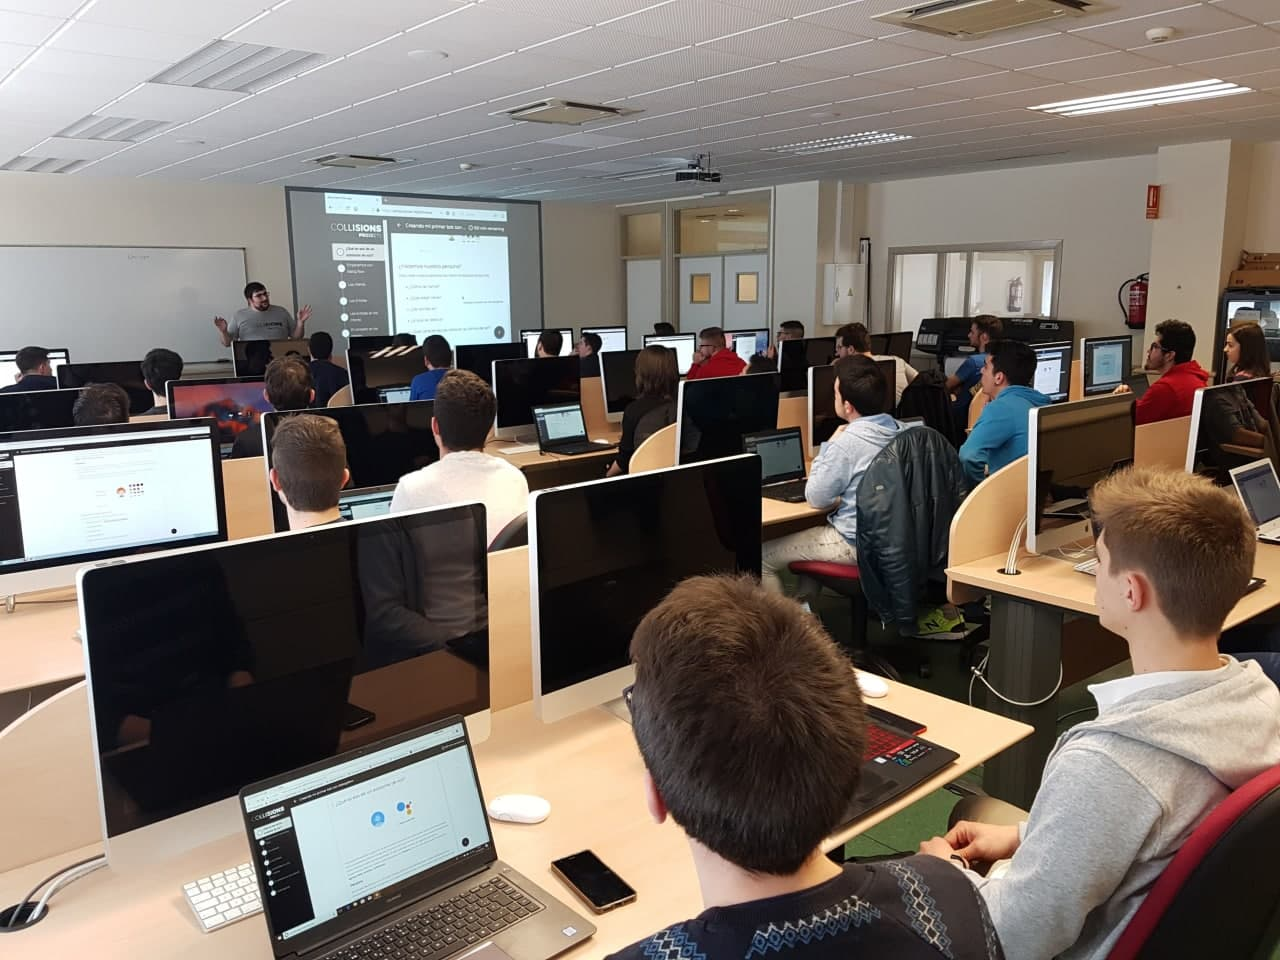
\includegraphics[width=0.6\textwidth]{Taller.jpg}
    \caption{Taller DevFest 2018}
    \label{fig:my_label}
\end{figure}


Gracias a el trato cercano que intentamos mantener con nuestros asistentes sabemos que las temáticas que hemos traído hasta ahora les han encantado. Esto no implica que en nuestro congreso no haya lugar para nuevas tecnologías emergentes o nuevas sugerencias.

\begin{figure}[h]
    \centering
    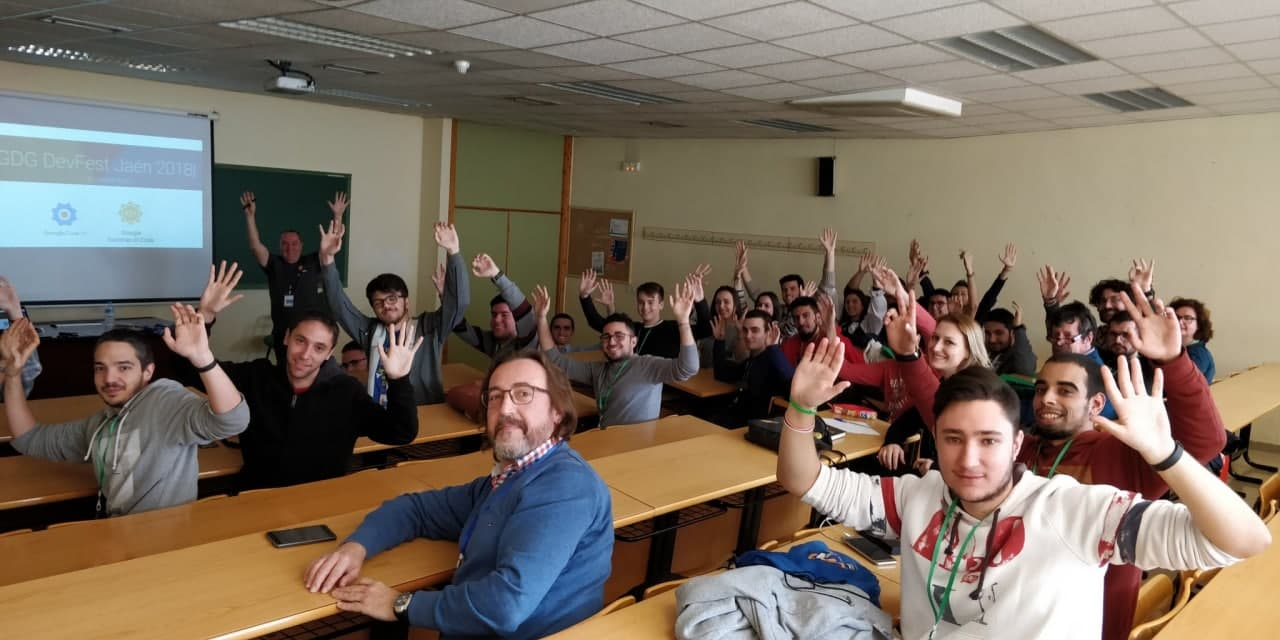
\includegraphics[width=0.6\textwidth]{Foto Charla.jpg}
    \caption{Charla Andreu Ibañez}
    \label{fig:my_label}
\end{figure}
\section{Lugar del Evento}

El evento será celebrado durante el día \textbf{11 de Diciembre de 2021} en la Universidad de Jaén, con horario por confirmar. La inauguración será en el edificio C1, donde se dará la bienvenida a los asistentes
y se llevarán a cabo las acreditaciones. Las charlas y los talleres se celebrarán en aulas del edificio C3 y los stands estarán colocados en el hall del edificio para que todos los asistentes los vean y puedan pasarse por ellos. 


\begin{figure}[h]
 \centering
  \subfloat[Edificio C3]{
   \label{f:gato}
    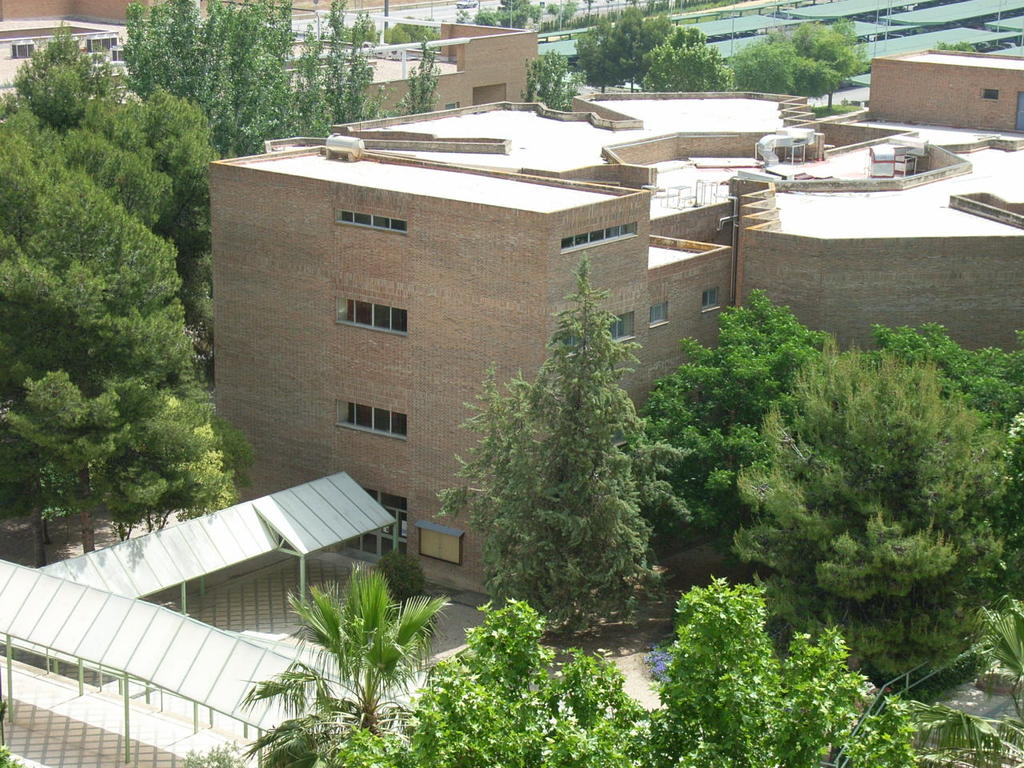
\includegraphics[width=0.45\textwidth]{ujaen3.jpg}}
  \subfloat[Plaza de los Pueblos]{
   \label{f:tigre}
    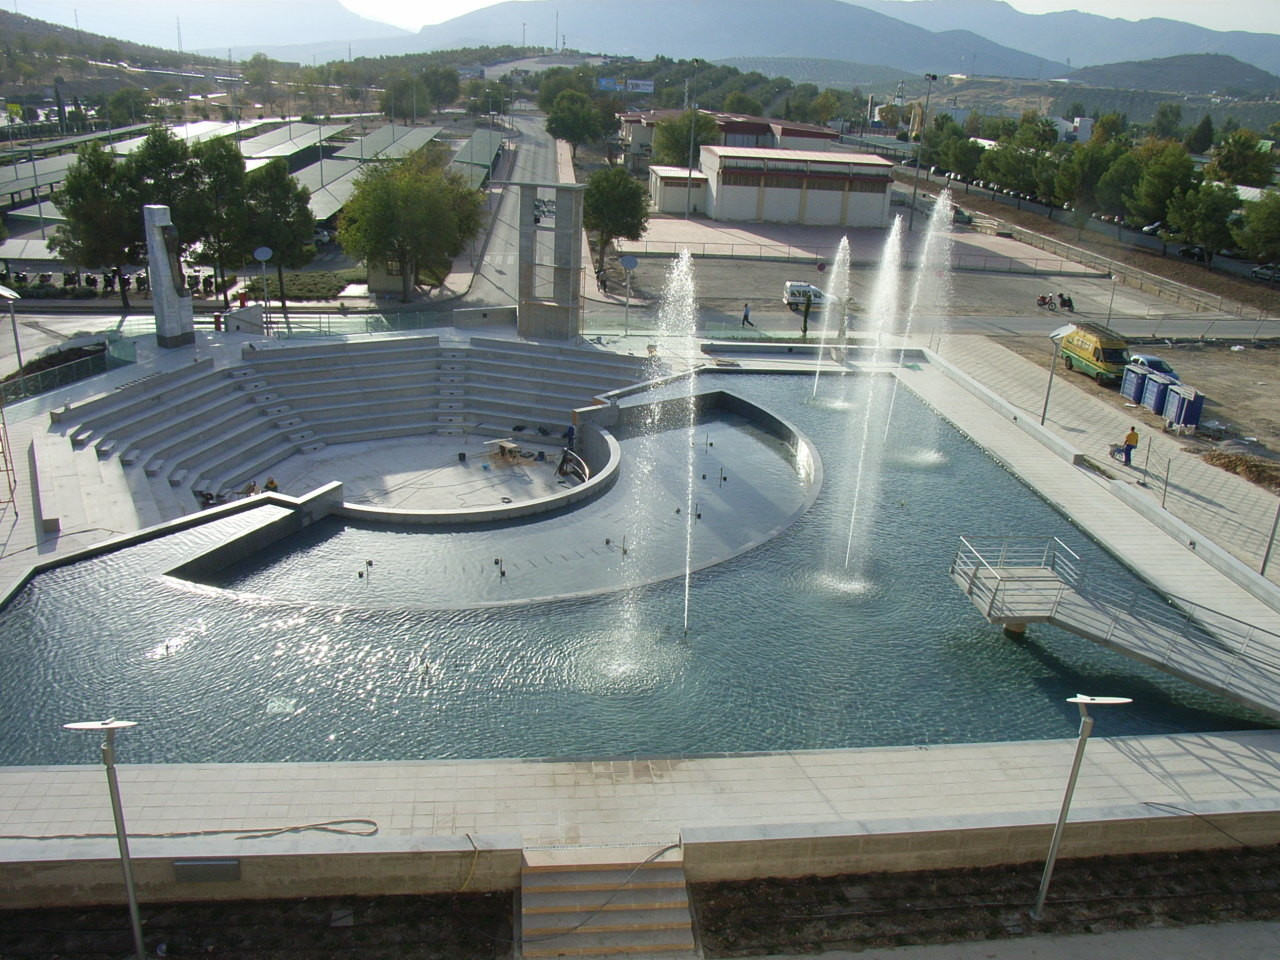
\includegraphics[width=0.45\textwidth]{ujaen2.jpg}}
 \caption{Universidad de Jaén}
 \label{f:animales}
\end{figure}

\section{Aforo}
 Debido a la Covid y al parón de la actividad dentro de la comunidad, se ha decidido reducir esta edición el aforo a sólo \textbf{250 personas}. Para ello, se ofrecen \textbf{tres aulas} con un aforo promedio de 100 personas para realizar las \textbf{charlas} en paralelo, una \textbf{cuarta} para los \textbf{talleres}, además de un aula de más de 300 personas de aforo para la inauguración y la clausura. 

\section{Patrocinios}

 Todo esto no se podría realizar sin el apoyo de empresas comprometidas con el desarrollo personal de la juventud jienense y, para poder ayudar en este proyecto, se han propuesto los siguientes escenarios.
 
 
 \begin{table}[ht]
 \centering
 \begin{tabular}{>{\centering\arraybackslash}m{3cm} >{\centering\arraybackslash}m{4cm} >{\centering\arraybackslash}m{2cm} >{\centering\arraybackslash}m{2cm} >{\centering\arraybackslash}m{2cm} }
   \toprule
    &  & 
\includegraphics[height=1cm]{diamante 2.png} & 
\includegraphics[height=1cm]{oro.png} & 
\includegraphics[height=1cm]{Plata.png} \\
   \midrule
          \textbf{Mecenazgo} &  & 1500\euro & 1000\euro & 600\euro \\
    %\hline
          \textbf{Ponencias} & Aula Grande & 
\includegraphics[height=1cm]{Tick Verde.png}& &\\
                    & Aula Pequeña & & 
\includegraphics[height=1cm]{Tick Verde.png}&
\includegraphics[height=1cm]{Tick Verde.png}\\
                    & Taller        &
\includegraphics[height=1cm]{Tick Verde.png} & 
\includegraphics[height=1cm]{Tick Verde.png}&\\
    %\hline
        \textbf{Stand}       & Grande        &
\includegraphics[height=1cm]{Tick Verde.png} & &\\
                    & Pequeño       & &
\includegraphics[height=1cm]{Tick Verde.png} &
\includegraphics[height=1cm]{Tick Verde.png}\\
    %\hline
        \textbf{Otros}      &Promoción      &
\includegraphics[height=1cm]{Tick Verde.png} &
\includegraphics[height=1cm]{Tick Verde.png} &
\includegraphics[height=1cm]{Tick Verde.png}\\
                    & Logo &
\includegraphics[height=1cm]{Tick Verde.png} &
\includegraphics[height=1cm]{Tick Verde.png} &
\includegraphics[height=1cm]{Tick Verde.png}\\
                    & Entrevista en vídeo   & 
\includegraphics[height=1cm]{Tick Verde.png}&
\includegraphics[height=1cm]{Tick Verde.png} &\\
                    & Grabar conferencias   & 
\includegraphics[height=1cm]{Tick Verde.png}& &\\
                    & Mención Notas Prensa & 
\includegraphics[height=1cm]{Tick Verde.png}& &\\
                    & Welcome Pack    & 
\includegraphics[height=1cm]{Tick Verde.png}& &\\
    \bottomrule
 \end{tabular}
 \caption{Patrocinios}
 \end{table}
 
 
\end{document}
